\newpage

\section{EAR - Eye Aspect Ratio}
Metoda polegająca na obliczeniu \textit{EAR}  \cite{EARRaspberryPi} \cite{eyeBlinkEARRosebrock}, czyli stosunek otwarcia oczu - wysokość do szerokości widocznej części gałki ocznej. Wykorzystuje się tu landmarki (patrz rozdz. \hyperref[{section:landmarks}]{\textit{\ref{section:landmarks}.Landmarks}}) naniesione dookoła oczu.

\subsection{Wzór obliczania EAR}
Zależnie od ilości punktów wokół oka będzie różny wzór obliczania EAR.\\
Dla 6 punktów:
\begin{align}
    EAR = \frac{dist(L_0, L_1) + dist(L_2, L4)}{2 * dist(L_3, L_5)}
\end{align}
\\
Natomiast, dla 4 punktów:
\begin{align}
    EAR = \frac{dist(L_0, L_2)}{dist(L_1, L_3)}
\end{align}

Gdzie \textit{$L_x$} to kolejne landmarki dokoła oczu, a \textit{dist} to odległość między dwoma punktami (odległość euklidesowa).\\

\subsection{Zasada działania EAR w kontekście mrugania}

W teorii otwarte oczy będą miały większy wymiar liczbowy EAR, niż oczy zamknięte. Na \hyperref[{fig:theoretical_eye_landmarks}]{\textit{rysunku \ref{fig:theoretical_eye_landmarks}}} widać, że oko otwarte ma większe odległości między punktami pionowymi niż w przypadku  oka zamkniętego. Dzięki takim różnicą możemy wykryć spadek wskaźnika EAR poniżej pewnego ustalonego poziomu oznaczający zamknięcie oka, natomiast wzrost otwarcie oka. Całościowo obserwując zmiany np. za pomocą pochodnej jesteśmy w stanie stwierdzić mrugnięcie.

\begin{figure}[!h]
    \begin{center}
        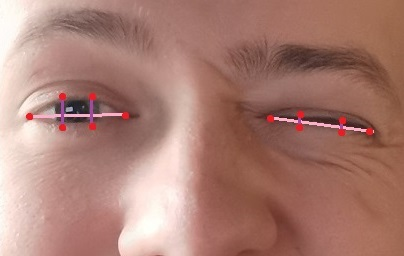
\includegraphics[scale=0.35]{img/landmark_section/theoretical_eye_landmarks.jpg}
        \caption{Teoretyczny rozmieszczene landmarków wokół oczu wraz z naniesionymi połączeniami do obliczenia EAR}
        \label{fig:theoretical_eye_landmarks}
    \end{center}
\end{figure}


\subsection{Testowanie z użyciem landmarków LBF opencv-contrib
}

\subsubsection{Test z użyciem kamery na żywo}

Wykonałem kilka krótkich testów z użyciem obrazu pochodzącego z przedniej kamery telefonu. 
\\
Poniżej znajdują się trzy testy, na których mrugnąłem tylko raz - lewym okiem, prawym i oboma na raz.

\begin{figure}[!h]
    \centering
    \begin{tikzpicture}
        \begin{axis}[
            xlabel = {Nr klatki obrazu z kamery},
            ylabel = {EAR},
            height = 0.5\linewidth,
            width = \linewidth,
            ymin= {0.10},
            ymax={0.30},
            ytick = {0.10, 0.12, 0.14, 0.16, 0.18, 0.20, 0.22, 0.24, 0.26, 0.28, 0.30},
            ymajorgrids = {true},
        ]
            \addplot[color=blue, mark=square*] table [x=x, y=a, col sep=comma] {csv/ear_left_1.csv};
            \addplot[color=red, mark=square*] table [x=x, y=b, col sep=comma] {csv/ear_left_1.csv};
        \end{axis}
    \end{tikzpicture}
    \caption{Mrugnięcie lewym okiem}
    \label{fig:left_eye_blink}
\end{figure}


\begin{figure}[!h]
    \centering
    \begin{tikzpicture}
        \begin{axis}[
            xlabel = {Nr klatki obrazu z kamery},
            ylabel = {EAR},
            height = 0.5\linewidth,
            width = \linewidth,
            ymin= {0.10},
            ymax={0.30},
            ytick = {0.10, 0.12, 0.14, 0.16, 0.18, 0.20, 0.22, 0.24, 0.26, 0.28, 0.30},
            ymajorgrids = {true},
        ]
            \addplot[color=blue, mark=square*] table [x=x, y=a, col sep=comma] {csv/ear_right_1.csv};
            \addplot[color=red, mark=square*] table [x=x, y=b, col sep=comma] {csv/ear_right_1.csv};
        \end{axis}
    \end{tikzpicture}
    \caption{Mrugnięcie prawym okiem}
    \label{fig:right_eye_blink}
\end{figure}

\begin{figure}[!h]
    \centering
    \begin{tikzpicture}
        \begin{axis}[
            xlabel = {Nr klatki obrazu z kamery},
            ylabel = {EAR},
            height = 0.5\linewidth,
            width = \linewidth,
            ymin= {0.10},
            ymax={0.30},
            ytick = {0.10, 0.12, 0.14, 0.16, 0.18, 0.20, 0.22, 0.24, 0.26, 0.28, 0.30},
            ymajorgrids = {true},
        ]
            \addplot[color=blue, mark=square*] table [x=x, y=a, col sep=comma] {csv/ear_both_1.csv};
            \addplot[color=red, mark=square*] table [x=x, y=b, col sep=comma] {csv/ear_both_1.csv};
        \end{axis}
    \end{tikzpicture}
    \caption{Mrugnięcie oboma oczami na raz}
    \label{fig:both_eyes_blink}
\end{figure}


Testy z pojedynczym mruganiem w krótkim okresie czasu dają przyzwoite wyniki i można na nich okreslić moment mrugania. W szczególności przy mrugnięciu jednym okiem.\\

Poniżej rozciągnąłem w czasie test na sekwencje kilku mrugnięć.

\begin{figure}[!h]
    \centering
    \begin{tikzpicture}
        \begin{axis}[
            xlabel = {Nr klatki obrazu z kamery},
            ylabel = {EAR},
            height = 0.5\linewidth,
            width = \linewidth,
            ymin= {0.10},
            ymax={0.30},
            ytick = {0.10, 0.12, 0.14, 0.16, 0.18, 0.20, 0.22, 0.24, 0.26, 0.28, 0.30},
            ymajorgrids = {true},
        ]
            \addplot[color=blue, mark=square*] table [x=x, y=a, col sep=comma] {csv/ear_long_1.csv};
            \addplot[color=red, mark=square*] table [x=x, y=b, col sep=comma] {csv/ear_long_1.csv};
        \end{axis}
    \end{tikzpicture}
    \caption{Kilka mrugnięć}
    \label{fig:multi_blinks_1}
\end{figure}

\begin{figure}[!h]
    \centering
    \begin{tikzpicture}
        \begin{axis}[
            xlabel = {Nr klatki obrazu z kamery},
            ylabel = {EAR},
            height = 0.5\linewidth,
            width = \linewidth,
            ymin= {0.10},
            ymax={0.30},
            ytick = {0.10, 0.12, 0.14, 0.16, 0.18, 0.20, 0.22, 0.24, 0.26, 0.28, 0.30},
            ymajorgrids = {true},
        ]
            \addplot[color=blue, mark=square*] table [x=x, y=a, col sep=comma] {csv/ear_long_2.csv};
            \addplot[color=red, mark=square*] table [x=x, y=b, col sep=comma] {csv/ear_long_2.csv};
        \end{axis}
    \end{tikzpicture}
    \caption{Kilka mrugnięć}
    \label{fig:multi_blinks_2}
\end{figure}

\begin{figure}[!h]
    \centering
    \begin{tikzpicture}
        \begin{axis}[
            xlabel = {Nr klatki obrazu z kamery},
            ylabel = {EAR},
            height = 0.5\linewidth,
            width = \linewidth,
            ymin= {0.10},
            ymax={0.30},
            ytick = {0.10, 0.12, 0.14, 0.16, 0.18, 0.20, 0.22, 0.24, 0.26, 0.28, 0.30},
            ymajorgrids = {true},
        ]
            \addplot[color=blue, mark=square*] table [x=x, y=a, col sep=comma] {csv/ear_long_3.csv};
            \addplot[color=red, mark=square*] table [x=x, y=b, col sep=comma] {csv/ear_long_3.csv};
        \end{axis}
    \end{tikzpicture}
    \caption{Kilka mrugnięć}
    \label{fig:multi_blinks_3}
\end{figure}

Tu również z dużym prawdopodobieństwem można okreśilć, w których klatkach wystąpiło mrugnięcie - widać gwałtowne obniżenie wartości EAR.
\\
Najlepsze wyniki były w przypadku pierwszego testu, ponieważ widać wtedy znaczną różnicę EAR między otwartym ($\sim0.26 - 0.30$), a zamkniętym okiem ($\sim0.12-0.18$). Na pozostałych testach różnice nie były już tak znaczące - na ostatnich dwóch wykresach otwarte i zamknięte oko ma niewielką różnicę w EAR. Takie małe różnice wyników mogą uniemożliwić prawidłową detekcję.

\vspace{3mm}
W każdym z przypadków testowych EAR dla jednego i drugiego oka prawie się pokrywają. Nawet przy mruganiu tylko jednym. Nie pozwoli to więc okręślić, którym okiem użytkownik mrugał.

\vspace{3mm}

Niewątpliwą trudnością w przypadku tej metody byłoby określenie progu wartości EAR, które zakwalifikowałbym jako mrugnięcie. Patrząc na wykresy powyżej można by przyjąć, że jest to wartość koło $~0.18$. Jednak w przypadku ostatecznego wyboru tej metody wymagałoby to dodatkowych badań celem określenia tej wartości.


\subsubsection{Niedokładność nakładania landmarków}

Patrząc jednak na położenie tych landmarków wokół oczu mam wątpliwości co do skuteczności tej metody:

\begin{figure}[!h]
    \begin{center}
        \subfigure[]{\label{fig:landmarks_accuracy_1}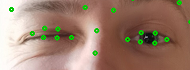
\includegraphics[scale=1.6]{img/landmark_section/landmarks_accuracy_1.png}}
        \hspace{8mm}
        \subfigure[]{\label{fig:landmarks_accuracy_2}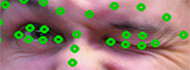
\includegraphics[scale=1.6]{img/landmark_section/landmarks_accuracy_2.png}}
    \end{center}
    \caption{Landmarki na oczach otwartych/zamkniętych}
    \label{fig:landmarks_accuracy_}
\end{figure}

Jak widać algorytm całkiem dobrze radzi sobie z rozmieszczeniem landmarków w przypadku otwartych oczu. Natomiast gdy oczy są zamknięte widać dużą niedokładność, która na pewno w dużym stopniu utrudnia prawidłową detekcję mrugnięcia.